
%\chapter{Planning Game World Structure}
%\label{sec:treehousearch}
 
  
%\section{Background}
%About patterns in city architecture and buildings
%patterns in biology 

%
%patterns in game worlds: dungeons
%


%In the next section I discuss literature on characteristics of succesfull leveldesign in games.  

\section{Considerations on Leveldesign in Games}


\chapter{Formalization of Game World Structure Patterns}
\label{sec:scenarios}


\section{Scenarios} 
In the next three sections we define game world scenarios that could occupate the generated forest structure. Each of the scenarios we propose here is based on a popular videogame genre: 

\begin{enumerate}
\item Puzzle / Adventure Dungeon
\item 3rd Person Strategy 
\item 1st Person Shooter
\end{enumerate} 


%\section{Scenario 1: Puzzle / Adventure Dungeon}
%Leveldesign Patterns in Puzzle and Adventure Dungeons:

%\begin{itemize}
%\item circular paths, loops. Example: The player arrives at a door and it is locked, you must take a different route and along the way you find a key. Now the player heads back to the door through which he can now proceed.  
%\item start at bottom, move to top. It is almost always the case that dungeons have multiple floors. The player starts at the bottom floor and progressing through %the dungeon means moving up to a higher floor.      
%\item re-using different paths by opening new door and locking old ones.    
%\item no path deviation. Rules for movement are very strict in these type of games.

%\end{itemize}

%\section{Planning Algorithm for Scenario 1}


%\section{Scenario 2: 3rd Person Strategy}


% hoe begint het algoritme?
% wat zijn de parameters? 
% 
%
%
%


%\section{Planning Algorithm for Scenario 2}

% hoe begint het algoritme?
% 
%
%
%
%


\section{The Scenario: 1st Person Shooter Multiplayer Arenas}

A first-person shooter is a game genre which centers the gameplay around gun- or projectile weapon-based combat through the first person perspective; i.e., the action is seen through the eyes of a protagonist, and thus the player. 


From this point on I will refer to this scenario as the 'Arena Scenario'.  


%\begin{figure}[ht]
%\centering
%\subfigure[]{
%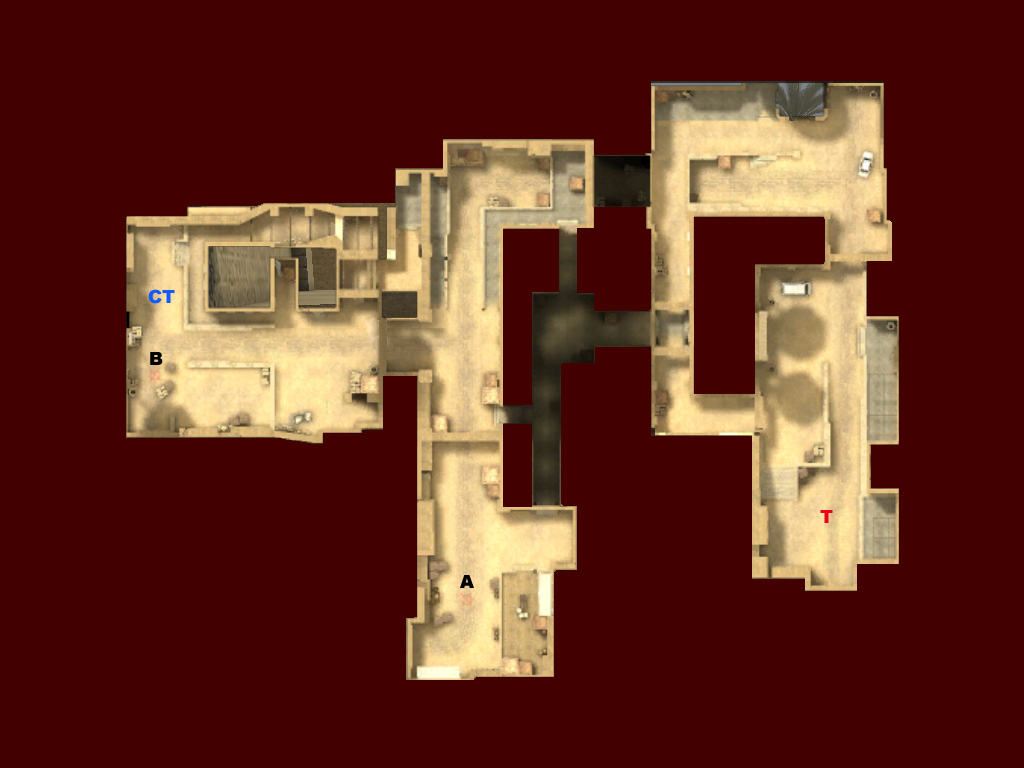
\includegraphics[width=300px]{images/game_maps/de_dust_overhead_2.jpg}
%\label{fig:subfig1}
%}
%\subfigure[]{
%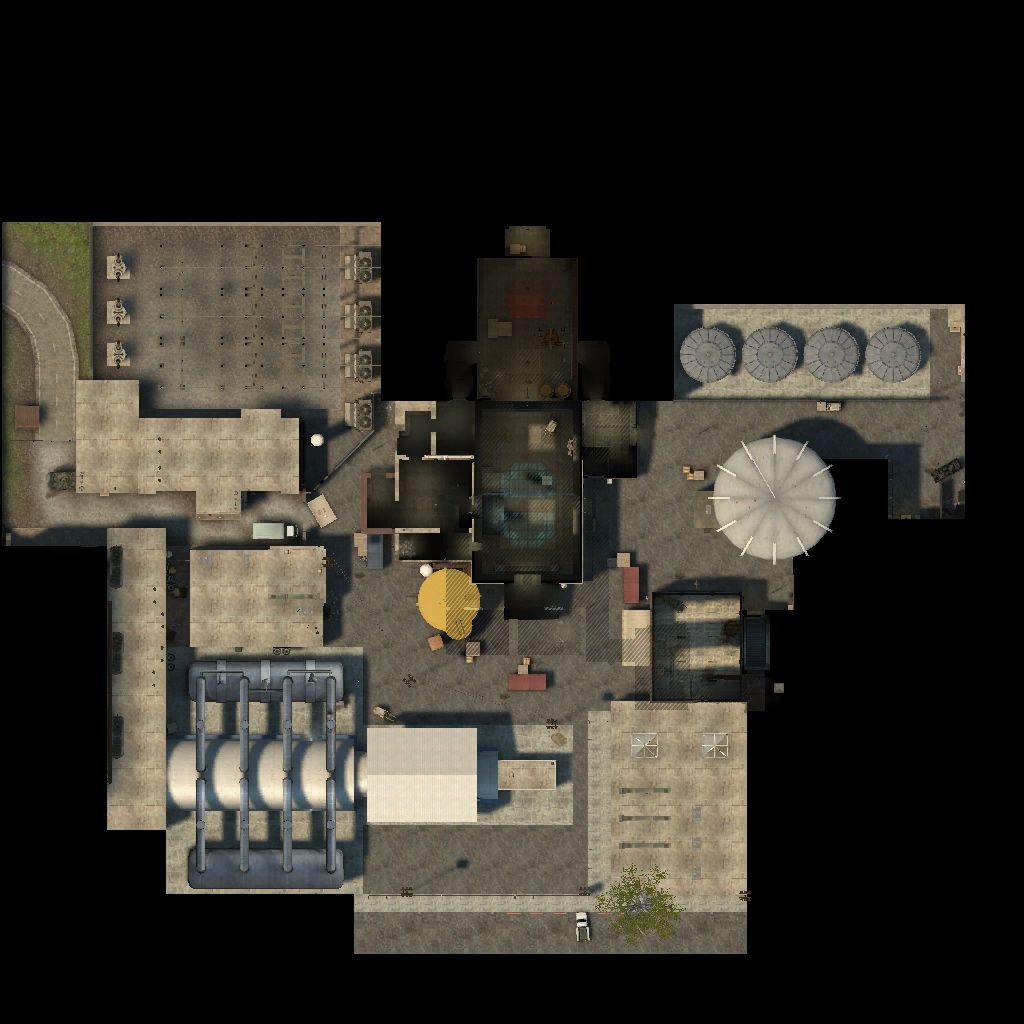
\includegraphics[width=300px]{images/game_maps/de_nuke.jpg}
%\label{fig:subfig2}
%}
%\label{fig:fpsmaps}
%\caption[Overview of classic FPS maps(from the game Counterstrike:Source). The "Multiple paths" pattern %is clearly visible.]{}
%\end{figure}

%\subsection{symmetry}

%\subsection{Multiple paths}

%\subsection{Local fights}

%\subsection{Collision points}

%\subsection{Reference points}
	
%\subsection{Defense areas}

%\subsection{Risk Incentive}



\subsection{Method for Finding Local Fight Points}

%randomization;

%patterns: symmetry patterns: 
%			polygonals: square, circle,
%

\subsection{Method for Finding Multiple Paths}

In this section I describe the $generateMultiplePaths()$ method for the generation of multiple paths to LFP's. This method should satisfy the 'Multiple Paths' pattern
of the \emph{Arena scenario}. Again note that there are two important graph structures: the $ForestGraph$ and the $MapGraph$. The initial state of the $ForestGraph$ holds all trees (vertices) and possible connections between trees (edges). The $MapGraph$ holds copies of all LFP vertices in the $ForestGraph$ which were found using the $findLFPs()$ method from the previous section. 

In the initial state all (LFP) vertices of the $MapGraph$ do not have any outgoing edges. For each LFP vertex in the $ForestGraph$ this method searches for the shortest path to all other reachable LFP's. Now we have found the shortest paths from every LFP vertex to any other LFP vertex, however we need alternative paths from a LFP to another LFP. So what follows is an iterative process to find alternative paths. In the first step the method found all shortest paths between LFPs. 
In the next step each shortest path is traversed and for every edge encountered, the edge's $traverse_rate$ property is increased by one. In this way we kan keep track of edges that are used by two or more shortest paths. The method stores the edges with highest $traverse_rate$ (edges that are used by the most shortest paths) in a list. When all shortest paths between LPF's have been traversed, the edges(with corresponding vertices) in the resulting list are copied to the $MapGraph$. After this step, the edges in the list are removed from the $ForestGraph$. In the next iteration the shortest paths will be alternatives since 1 or more edges of the shortest paths from the previous iteration have been removed from the graph. If all LFP's are unconnected with respect to other LFP's in the $ForestGraph$ we proceed to the next step; which is connecting all unconnected subgraphs to form a single connected graph.       

%todo: waarom?%
         

%algorithm outline








%\section{Planning Algorithm for Scenario 3}

% hoe begint het algoritme?
% 
%
%
%
%

%From the scenarios I discussed in the previous section we can extract a set of parameters and goals for our algorithms.
\chapter{Planning Algorithms}

\section{Considerations}

\section{Planning Methods}

%
%
%
%
\label{sec:PlanningAlgorithm} 
  
 Using the scenarios and architectural elements we have defined in the previous section we will formulate our planning algorithm now.
 I will first introduce the planning algorithm informally followed by a more formal approach.
      
  
%\begin{algorithm}
%\caption{The planning algorithm}
%\begin{algorithmic}
%\IF {$i\geq maxval$} 
%        \STATE $i\gets 0$
%\ELSE
%        \IF {$i+k\leq maxval$}
%                \STATE $i\gets i+k$
%        \ENDIF
%\ENDIF 
%\end{algorithmic}
%\end{algorithm}


\chapter{Geometry Generation}

\section{Procedural Generation of Architecture Geometry} 
\label{sec:archelements}
 
%nog iets moois hiervoor 
In this section we present the geometrical elements we use for the construction of our treebased architecture. We will first introduce the elements in a broad sense, followed by descriptions of methods to construct the geometry of some of these elements procedurally. 
 
\subsection{The Element Vocabulary}
We established a set of architectural elements we believe are the most basic tree-based architectural structures: 

\begin{enumerate}
\item Platforms
\item Buildings
\item Bridges 
\item Stairs
\item Miscellaneous Elements 
\end{enumerate} 

\begin{figure}[ht]
\centering
\subfigure[Platform]{
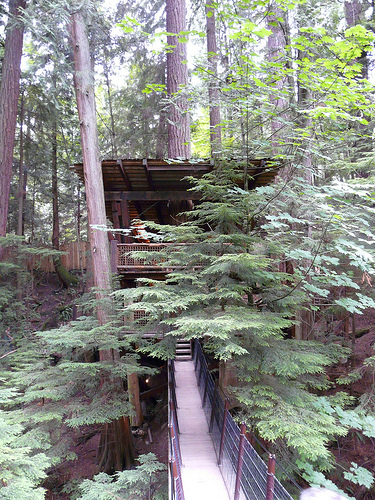
\includegraphics[width=50px]{images/platform.jpg}
\label{fig:subfig1}
}
\subfigure[House]{
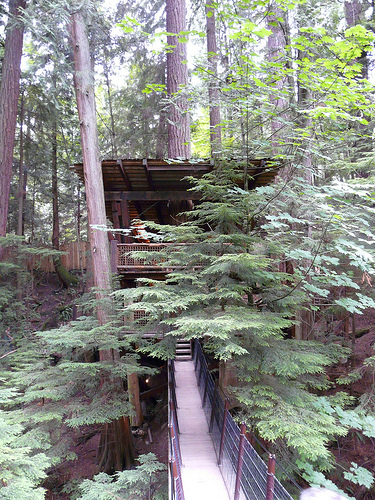
\includegraphics[width=50px]{images/house.jpg}
\label{fig:subfig2}
}
\subfigure[Bridge]{
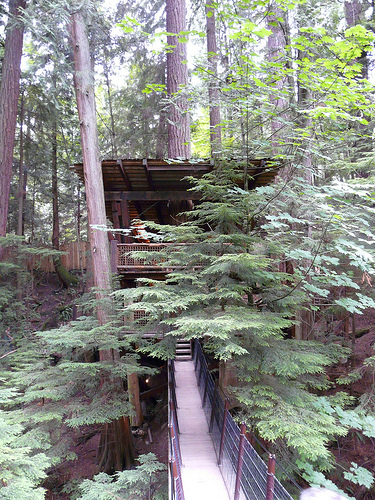
\includegraphics[width=50px]{images/bridge.jpg}
\label{fig:subfig3}
}
\subfigure[Stairs]{
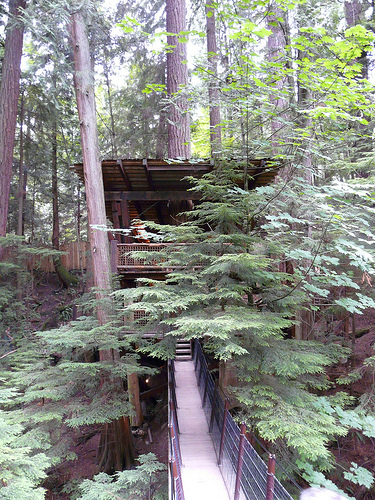
\includegraphics[width=50px]{images/stairs.jpg}
\label{fig:subfig3}
}
\label{fig:archElements}
\caption[Architectural Elements Vocabulary]{Caption of subfigures \subref{fig:subfig1}, \subref{fig:subfig2} and \subref{fig:subfig3}}
\end{figure}


 
\subsection{Platforms}
\label{sec:platform}
 


\subsection{Housing}
\label{sec:building}




\subsection{Bridges}
\label{sec:bridges}





\begin{figure}[ht]
\centering
\includegraphics[width=200px]{images/suspension-bridge.jpg}
\label{fig:bridgeExample}
\caption{A typical suspension bridge}
\end{figure}
The curved surface of a suspension bridge can easily be described with a spline.   

\subsection{Stairs}
\label{sec:stairs}
  
We define two types of stairs. The first is the simple vertical linear stairs-type. The second is the revolving staircase, which revolves around a tree trunk like a corkskrew. 


%\subsection{Connecting Elements} 
%
%We construct an architectural structure by combining the elements we have in our element vocabulary.
%In order to construct logical combinations we need to define for each elements how it can be joined with other elements
%in our vocabulary.

  
